% /**
% * Copyright 2012 Sergio García Mondaray
% *
% * This file is part of GodTIC-Templates (www.godtic.com).
% * 
% * GodTIC-Templates is free software: you can redistribute it and/or modify it
% * under the terms of the GNU General Public License as published by
% * the Free Software Foundation (version 3 of the License).
% * 
% * GodTIC-Templates is distributed in the hope that it will be useful, but
% * WITHOUT ANY WARRANTY; without even the implied warranty 
% * of MERCHANTABILITY or FITNESS FOR A PARTICULAR PURPOSE. 
% * See the GNU General Public License for more details.
% * 
% * You should have received a copy of the GNU General Public License 
% * along with GodTIC-Templates. If not, see http://www.gnu.org/licenses/.
% **/
%%%%%%%%%%%%%%%%%%%%%%%%%%%%%%%%%%%%%%%%%%%%%%%%%%%%%%%%%%%%%%%%%%%%%%
\documentclass[12pt]{beamer}% /**
% * Copyright 2012 Sergio García Mondaray
% *
% * This file is part of GodTIC-Templates (www.godtic.com).
% * 
% * GodTIC-Templates is free software: you can redistribute it and/or modify it
% * under the terms of the GNU General Public License as published by
% * the Free Software Foundation (version 3 of the License).
% * 
% * GodTIC-Templates is distributed in the hope that it will be useful, but
% * WITHOUT ANY WARRANTY; without even the implied warranty 
% * of MERCHANTABILITY or FITNESS FOR A PARTICULAR PURPOSE. 
% * See the GNU General Public License for more details.
% * 
% * You should have received a copy of the GNU General Public License 
% * along with GodTIC-Templates. If not, see http://www.gnu.org/licenses/.
% **/

\usepackage[utf8]{inputenc}
\usepackage[spanish]{babel}

\usetheme{/theme}
\usepackage{thumbpdf}
\usepackage{wasysym}
\usepackage{ucs}
\usepackage{pgf,pgfarrows,pgfnodes,pgfautomata,pgfheaps,pgfshade}
\usepackage{verbatim}
\usepackage{hyperref}
\usepackage{pifont}
\usepackage{color}
\usepackage{wrapfig}
\usepackage{graphicx}
\definecolor{mygreen}{rgb}{0,0.7,0.1}
\definecolor{myorange}{rgb}{1,0.5,0}

\graphicspath{{img/}} 
\DeclareGraphicsExtensions{.pdf,.png,.jpg}
\usepackage{listings}

\usepackage{color}
\definecolor{lightgray}{rgb}{.9,.9,.9}
\definecolor{darkgray}{rgb}{.4,.4,.4}
\definecolor{purple}{rgb}{0.65, 0.12, 0.82}

\lstdefinelanguage{JavaScript}{
  keywords={typeof, new, true, false, catch, function, return, null, catch, switch, var, if, in, while, do, else, case, break},
  keywordstyle=\color{blue}\bfseries,
  ndkeywords={class, export, boolean, throw, implements, import, this},
  ndkeywordstyle=\color{darkgray}\bfseries,
  identifierstyle=\color{black},
  sensitive=false,
  comment=[l]{//},
  morecomment=[s]{/*}{*/},
  commentstyle=\color{purple}\ttfamily,
  stringstyle=\color{red}\ttfamily,
  morestring=[b]',
  morestring=[b]"
}

\lstset{tabsize=4,
  showspaces=false,
  showtabs=false,
  frame=l,
  framerule=1pt,
  aboveskip=0.5cm,
  framextopmargin=3pt,
  framexbottommargin=3pt,
  framexleftmargin=18pt,
  framesep=.4pt,
  rulesep=.4pt,
  stringstyle=\ttfamily,
  showstringspaces = false,
  basicstyle=\footnotesize\ttfamily,
  keywordstyle=\bfseries,
  numbers=left,
  numbersep=6pt,
  numberstyle=\color[cmyk]{0.43, 0.35, 0.35,0.01}\bfseries\scriptsize\ttfamily,
  numberfirstline = true,
  breaklines=true,
  stepnumber=1,
  backgroundcolor=\color{white},
  xleftmargin=18pt,
  framexrightmargin=0pt,
  xrightmargin=0pt,
  language=JavaScript
}
 %%%%%% METADATOS %%
%%%%%%%%%%%%%%%%%%%%%%%%%%%%%%%%%%%%%%%%%%%%%%%%%%%%%%%%%%%%%%%%%%%%%%

\def\titulo{
  Grampus, el FOCA para Linux
}
\def\autor{
  Jose Moruno Cadima
}
\def\email{
  snifer@h-sec.org
}
\date{Hackmeeting 2013} % (Opcional) Puede tener varias líneas, estilos, etc

%%%%%%%%%%%%%%%%%%%%%%%%%%%%%%%%%%%%%%%%%%%%%%%%%%%%%%%%%%%%%%%%%%%%%%
\begin{document}% /**
% * Copyright 2012 Sergio García Mondaray
% *
% * This file is part of GodTIC-Templates (www.godtic.com).
% * 
% * GodTIC-Templates is free software: you can redistribute it and/or modify it
% * under the terms of the GNU General Public License as published by
% * the Free Software Foundation (version 3 of the License).
% * 
% * GodTIC-Templates is distributed in the hope that it will be useful, but
% * WITHOUT ANY WARRANTY; without even the implied warranty 
% * of MERCHANTABILITY or FITNESS FOR A PARTICULAR PURPOSE. 
% * See the GNU General Public License for more details.
% * 
% * You should have received a copy of the GNU General Public License 
% * along with GodTIC-Templates. If not, see http://www.gnu.org/licenses/.
% **/


\author{\autor}
\title{\titulo}

\frame{\titlepage}

\section*{}
\begin{frame}
  \frametitle{Índice}
  \framesubtitle{Contenido de la presentación}
  \tableofcontents[section=1,hidesubsections]
\end{frame}
\AtBeginSection[]
{
  \frame<handout:0>
  {
    \frametitle{Índice}
    \framesubtitle{Contenido de la presentación}

    \tableofcontents[currentsection,hideallsubsections]
  }
}
\AtBeginSubsection[]
{
  \frame<handout:0>
  {
    \frametitle{Índice}
    \framesubtitle{Contenido de la presentación}
    \tableofcontents[sectionstyle=show/hide,subsectionstyle=show/shaded/hide]
  }
}
\newcommand<>{\highlighton}[1]{
  \alt#2{\structure{#1}}{{#1}}
}
\newcommand{\icon}[1]{\pgfimage[height=1em]{#1}}

%% Título y subtítulo

\def\frametit{\insertsection}
\def\framesubtit{\insertsubsection}

%\newcommand{\slide}[1]{\begin{frame}\frametitle{\frametit}\framesubtitle{\framesubtit}#1\end{frame}}

\newenvironment{slide}[1][]
  {\begin{frame}[fragile,environment=slide,#1]
    \frametitle{\frametit}\framesubtitle{\framesubtit}}
  {\end{frame}}

\newenvironment{blankslide}[1][]
  {\begin{frame}[fragile,environment=blankslide,#1]
    \frametitle{}\framesubtitle{}}
  {\end{frame}}

%\newenvironment{slide}{\begin{frame}}{\end{frame}}
% \newenvironment{slidef}{\begin{xframe}}{\end{xframe}}
 %%%%%%%%% INICIO DEL DOCUMENTO %%
%%%%%%%%%%%%%%%%%%%%%%%%%%%%%%%%%%%%%%%%%%%%%%%%%%%%%%%%%%%%%%%%%%%%%%

%%%%%%%%%%%%%%%%%%%%%%%%%%%%%%%%%%%%%%%%%%%%%%%%%%%%%%%%%%%%%%%%%%%%%%
\begin{document}% /**
% * Copyright 2012 Sergio García Mondaray
% *
% * This file is part of GodTIC-Templates (www.godtic.com).
% * 
% * GodTIC-Templates is free software: you can redistribute it and/or modify it
% * under the terms of the GNU General Public License as published by
% * the Free Software Foundation (version 3 of the License).
% * 
% * GodTIC-Templates is distributed in the hope that it will be useful, but
% * WITHOUT ANY WARRANTY; without even the implied warranty 
% * of MERCHANTABILITY or FITNESS FOR A PARTICULAR PURPOSE. 
% * See the GNU General Public License for more details.
% * 
% * You should have received a copy of the GNU General Public License 
% * along with GodTIC-Templates. If not, see http://www.gnu.org/licenses/.
% **/


\author{\autor}
\title{\titulo}

\frame{\titlepage}

\section*{}
\begin{frame}
  \frametitle{Índice}
  \framesubtitle{Contenido de la presentación}
  \tableofcontents[section=1,hidesubsections]
\end{frame}
\AtBeginSection[]
{
  \frame<handout:0>
  {
    \frametitle{Índice}
    \framesubtitle{Contenido de la presentación}

    \tableofcontents[currentsection,hideallsubsections]
  }
}
\AtBeginSubsection[]
{
  \frame<handout:0>
  {
    \frametitle{Índice}
    \framesubtitle{Contenido de la presentación}
    \tableofcontents[sectionstyle=show/hide,subsectionstyle=show/shaded/hide]
  }
}
\newcommand<>{\highlighton}[1]{
  \alt#2{\structure{#1}}{{#1}}
}
\newcommand{\icon}[1]{\pgfimage[height=1em]{#1}}

%% Título y subtítulo

\def\frametit{\insertsection}
\def\framesubtit{\insertsubsection}

%\newcommand{\slide}[1]{\begin{frame}\frametitle{\frametit}\framesubtitle{\framesubtit}#1\end{frame}}

\newenvironment{slide}[1][]
  {\begin{frame}[fragile,environment=slide,#1]
    \frametitle{\frametit}\framesubtitle{\framesubtit}}
  {\end{frame}}

\newenvironment{blankslide}[1][]
  {\begin{frame}[fragile,environment=blankslide,#1]
    \frametitle{}\framesubtitle{}}
  {\end{frame}}

%\newenvironment{slide}{\begin{frame}}{\end{frame}}
% \newenvironment{slidef}{\begin{xframe}}{\end{xframe}}
 %%%%%%%%% INICIO DEL DOCUMENTO %%
%%%%%%%%%%%%%%%%%%%%%%%%%%%%%%%%%%%%%%%%%%%%%%%%%%%%%%%%%%%%%%%%%%%%%%
\section{Whoami}

\begin{slide}
  
    \begin{figure}[h]
      \begin{center}
        
\includegraphics[height=0.5\textheight]{img/sniferl4bs.png}
Jose Moruno Cadima A.K.A Snifer\pause
      \end{center}
    \end{figure}
  \begin{itemize}
  \item Consultor, Analisis de Malware, Android .\pause
  \item Desarrollador en Python, Perl, Ruby.\pause
  \item Integrante de Uremix, HackLab Cochabamba, Grampus Team.\pause
  \end{itemize}
\end{slide}
\section{Introducción}

%%

\subsection{Que es Grampus}
\begin{slide}
	\begin{enumerate}  
  	  \item Herramienta desarrollada en Python.\pause
 	  \item Open Source.\pause
 	  \item Alternativa a la Foca.\pause
 	  \item Se encuentra en fase Beta.\pause
 	  \item Multiplataforma.
        \end{enumerate}
\end{slide}



\subsection{Que es La Foca}

%%

\begin{slide}
	\begin{enumerate}  
  	  \item Herramienta desarrollada con .Net\pause
 	  \item Software de Pago, teniendo una versión de Pago  y otra con limitaciones.\pause
 	  \item No corre en Linux, se tiene que pelear con WINE para su funcionamiento.\pause
 	  \item Solo para Windows
        \end{enumerate}
\end{slide}
%%

\begin{slide}
  GRAMPUS TEAM esta conformado
  \begin{enumerate}
  \item Sanko.\pause
  \item Prop3th.\pause
  \item 11Sept.\pause
  \item Overflow.\pause
  \item Snifer (Jose Moruno Cadima).\pause
  \end{enumerate}
\end{slide}

%%

\subsection{Porque Python}

\begin{slide}
  Se eligio Python, porque es un lenguaje multiplataforma, adaptable  a nuestras necesidades lenguaje que mejor nos manejos los integrantes del equipo.
 

    \begin{figure}[h]
      \begin{center}
        
\includegraphics[height=0.5\textheight]{img/grampu.jpg}
      \end{center}
   \end{figure}
\end{slide}

%
\subsection{Porque nace Grampus}
%

\begin{slide}
 Grampus nace, por ......
    \begin{figure}[h]
      \begin{center}
        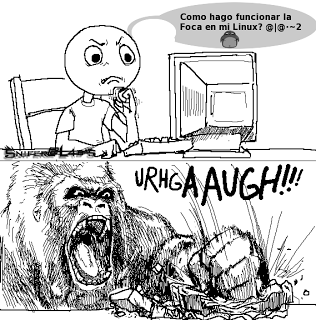
\includegraphics[height=0.7\textheight]{img/byeFOca.png}
        \caption{Pelea con la Foca}
        \label{fig::uclm}
      \end{center}
   \end{figure}
\end{slide}


%%

\subsection{Grampus Project}
  \begin{slide} 
 	\begin{itemize}
  	 \item Grampus.\pause
  	 \item Anti-Grampus.\pause
 	 \item Forensic Grampus.\pause
 	 \item Anti-Forensic Grampus.
  \end{itemize}
\end{slide}



\subsection{Una pasada a los módulos}
\begin{slide} 
  \begin{exampleblock}{Grampus}
    Herramienta de Footprintig  y analisis de metadata. \pause
  \end{exampleblock}

  \begin{exampleblock}{Anti - Grampus}
     Cambio de Metadata con información, no relevante.\pause
  \end{exampleblock}

\end{slide}


\subsection{Una pasada a los módulos}
\begin{slide}
  
  \begin{exampleblock}{Forensic Grampus}
    Volcado de Memoria RAM, File Carving, Recuperación de Información .\pause
  \end{exampleblock}

  \begin{exampleblock}{Anti-Forensic Grampus}
    Borrado seguro de información, Sobreescribimiento. \pause
  \end{exampleblock}
\end{slide}

%
\subsection{Proyecto relacionado Clean Box}
\begin{slide}
  \begin{itemize}
  \item Servicio Web, Open Source.\pause
  \item Actuando como un filtro para DropBox el MITM de la red :D.\pause
  \item Trabajar directamente con un servidor, el cual brinde la opción del eliminado de los metadatos.
  \end{itemize}
\end{slide}
%
\subsection{Objetivos del Proyecto}
\begin{slide} 
  \begin{exampleblock}{}
    Como desarrolladores nuestro objetivo sería la implementación de nuevas tareas para la recopilación de información y el mantenimiento de los bugs que vayan saliendo. \pause
  \end{exampleblock}

  \begin{exampleblock}{}
   Fuera de eso, queremos incentivar el desarrollo colectivo para que esta herramienta pueda ir automanteniendose y autorenovandose gracias a la colaboración de desarrolladores que usen la herramienta y así conseguir el objetivo común de una herramienta multiplataforma, estable y eficiente. \pause
  \end{exampleblock}

  \begin{exampleblock}{}
   Que el proyecto se centre en un eje de colaboración colectiva, automantenerse entre todos los desarrolladores de Python.
  \end{exampleblock}
\end{slide}


%

%%

\section{GRAMPUS FASE BETA! :( }
\begin{figure}[h]
      \begin{center}
        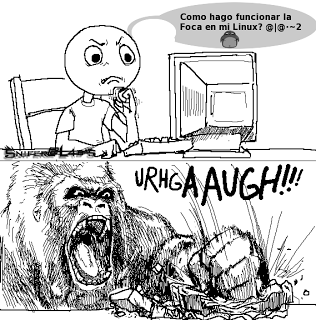
\includegraphics[height=0.7\textheight]{img/byeFOca.png}
        \caption{Pelea con la Foca}
        \label{fig::uclm}
      \end{center}
   \end{figure}

  \begin{slide} 
	Grampus es una herramienta dirigida especialmente a analistas forenses y a pentesters en general, en su primera fase la cual es BETA cuenta con las   	siguientes características.
\end{slide}
%%

\begin{slide}
  \begin{itemize}
  \item Extracción de metadatos de documentos e imágenes, formatos soportados : Openoffice/Libreoffice, Office 2007, Office 2003, PDF, jpg, flv y gif.\pause
  \item Eliminación de metadatos extraidos de diferentes documentos e imágenes.\pause
  \item Tres tipos de Crawlers, entre los que se encuentra un crawler de documentos (por extensión) usando Google hacking.\pause
  \item Para la tarea del fingerprinting contamos con un server banner y un escaneo mediante Shodan usando su api
  \end{itemize}
\end{slide}

%%

\subsection{Bugs Conocidos}

%%

\begin{slide}

  \begin{block}{Directorios}
    Abriendo un directorio, todos los metadatos en el último tab.\pause
  \end{block}

  \begin{alertblock}{Problemas de Instalación}
    Problemas con setup.py el instalador anda de pocas malas bien.\pause
  \end{alertblock}

  \begin{exampleblock}{Problemas con la Araña}
    De nuez en cuando funciona correctamente.
  \end{exampleblock}

\end{slide}

%

\section{ Donde anda Grampus ahora! }
\begin{figure}[h]
      \begin{center}
        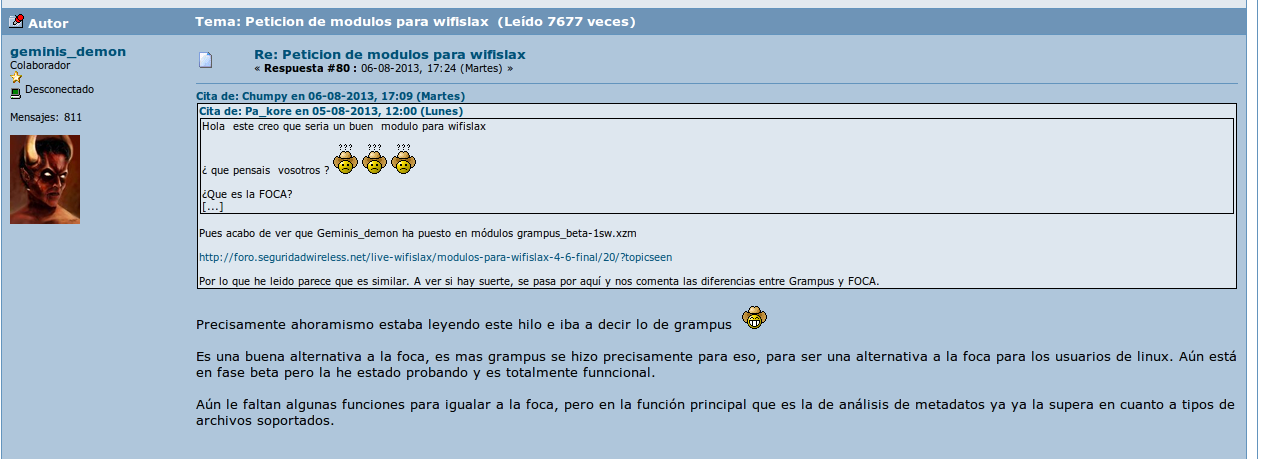
\includegraphics[height=0.7\textheight]{img/wifislax.png}
        \caption{WIFISLAX}
        \label{fig::uclm}
      \end{center}
   \end{figure}

%

\section{Conocer mas sobre Grampus }

%%

\begin{slide}
  \begin{thebibliography}{9}

  \bibitem{}
    Blog Personal - www.sniferl4bs.com 
    \emph{Snifer@L4bs}.


  \bibitem{}
    Repositorio Oficial,
    \emph{BitBucket}.
    www.bitbucket/grampusteam/


  \end{thebibliography}

\end{slide}

%%%%%%%%%%%%%%%%%%%%%%%%%%%%%%%%%%%%%%%%%%%%%%%%%%%%%%%%%%%%%%%%%%%%%%
%%%%%%%%%%%%%%%%%%%%%%%%%%%%%%%%% FIN %%%%%%%%%%%%%%%%%%%%%%%%%%%%%%%%
%%%%%%%%%%%%%%%%%%%%%%%%%%%%%%%%%%%%%%%%%%%%%%%%%%%%%%%%%%%%%%%%%%%%%%

\begin{blankslide}
  \vspace{1cm}
  \begin{center}
    {\Large Gracias por su atención}
  \end{center}
  \vspace{1cm}
  \begin{flushright}
    {\bf \autor}\\
    {\tt \email}\\[0.5cm]

    {\scriptsize Twitter: @sniferl4bs}
    {\scriptsize WEB: sniferl4bs.com}
    {\scriptsize Presentación compuesta con \LaTeX }
  \end{flushright}
\end{blankslide}

\end{document}
